\chapter{Interface gráfica e arquitetura Web}
\label{cap:interface}

A aplicação segue uma arquitetura cliente-servidor. O servidor, em Java~17 (ou
superior) com Spring Boot 3.3.4, corre a simulação e o motor de inferência. O
cliente é uma aplicação Angular~18 que só apresenta o estado e envia comandos. A
interface nunca avalia condições de condução: as distâncias de segurança, os
limites de velocidade e a segurança das mudanças de faixa são decididos apenas
no motor de regras. A interface limita-se a desenhar as coordenadas que o
servidor envia.

A comunicação usa dois canais. Os comandos seguem por REST, cada um com a sua
resposta: iniciar, parar ou reiniciar a simulação, escolher um cenário,
acrescentar elementos à estrada e trocar de motor. O estado da simulação chega
por um WebSocket (\cod{/api/ws/simulation}). O servidor publica um
\emph{snapshot} em JSON a cada ciclo de 100\,ms, que é o mesmo conteúdo que a
API REST devolve. Se a ligação cair ou deixar de receber dados, o cliente volta
a ligar-se.

A interface (\cref{fig:interface-web}) mostra a estrada em perspetiva, com o
veículo, os outros atores, a sinalização e a meteorologia. Mostra também a decisão atual e as propostas
concorrentes, cada uma com o seu resultado na arbitragem. Os restantes painéis
apresentam a regra de origem, a razão e a evidência, a linha temporal das regras
e dos factos, a memória de trabalho e as leituras dos sensores.

Uma biblioteca de cenários e uma caixa de ferramentas permitem montar situações
durante a execução: veículos, peões, sinais, semáforos, buracos, obstáculos,
barreiras e chuva. Um seletor troca entre os motores Drools e Prolog,
recarregando o cenário. Se o motor falhar, um aviso mostra a mensagem de erro.
O diálogo de perguntas \emph{Why}, \emph{Why not} e \emph{How}, que abre
quando a simulação para, é descrito na \cref{sec:expl-registo}.

\begin{figure}[H]
  \centering
  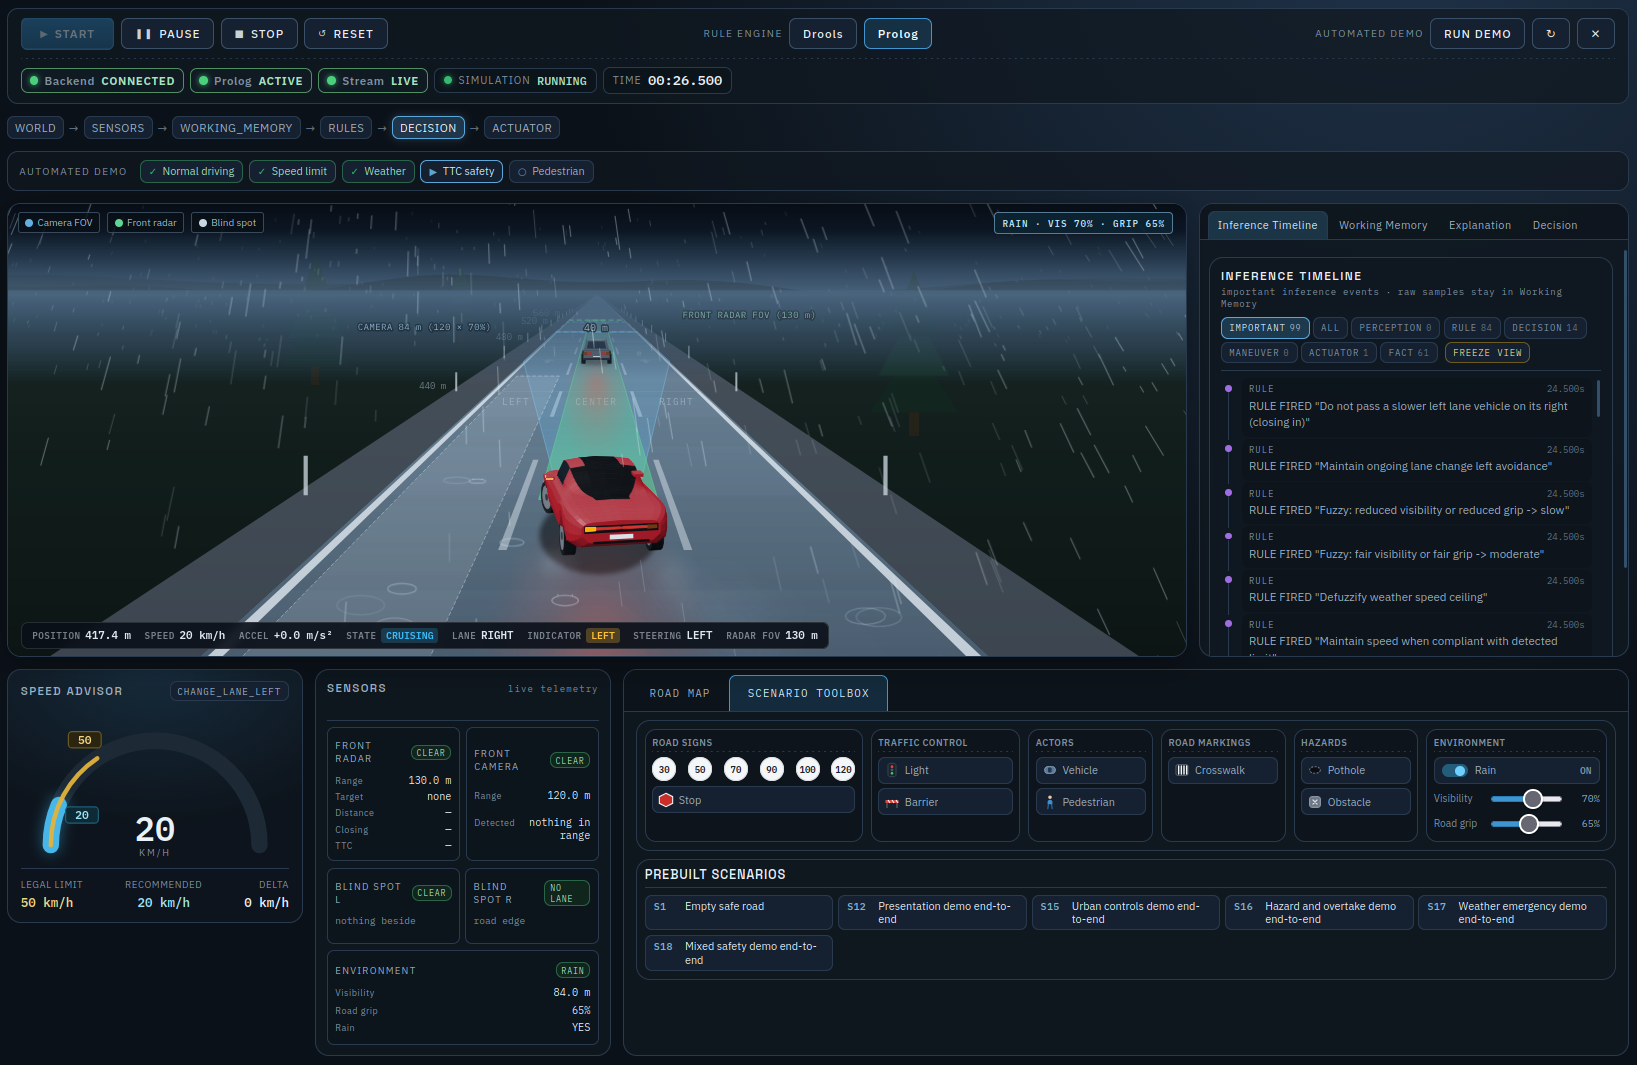
\includegraphics[width=0.85\textwidth]{figuras/screenshot-web-ui.png}
  \caption{Interface Web com o motor Prolog ativo, durante uma ultrapassagem com chuva.}
  \label{fig:interface-web}
\end{figure}
